% \documentclass[conference]{IEEEtran}

\usepackage{cite}
\usepackage{amsmath,amssymb,amsfonts}
\usepackage[english]{babel}
\usepackage{algorithmic}
\usepackage{graphicx}
\usepackage{textcomp}
\usepackage{xcolor}

% \def\BibTeX{{\rm B\kern-.05em{\sc i\kern-.025em b}\kern-.08em
%     T\kern-.1667em\lower.7ex\hbox{E}\kern-.125emX}}




\title{Projet d'identification du pendule inverse
% {\footnotesize \textsuperscript{}
}

% \author{
%     \IEEEauthorblockN{Adrien \textsc{Pétard} (3809346)}
%     % A la ligne:

%     % \IEEEauthorblockA{Master SAR\\
%     %     \textit{Student number 3809346}
%     % }
% }
\author{Adrien \textsc{Pétard} (3809346)}
    % A la ligne:

    % \IEEEauthorblockA{Master SAR\\
    %     \textit{Student number 3809346}
    % }



\begin{document}
\maketitle

\begin{abstract}
    Dans ce document, nous allons étudier la modélisation d'un systèmes, le Qube-Servo 2, avec un disque simple et un pendule inversé. \\
    Nous allons étudier les paramètres du moteur, puis affiner les paramètres du modèle. Enfin, nous allons étudier la modélisation du pendule inversé.\\
    Nous allons utiliser le logiciel Matlab->Simulink pour réaliser les simulations et les calculs.\\
    Notre objectif est de comparer les données de simulation avec des données réelles acquises sur la maquette.
    Pour cela, nous allons passer par une identfification des paramètres physiques du modèle, \\
    Puis nous modifierons les paramètres du modèle pour obtenir une simulation la plus proche possible des données réelles et ainsi améliorer la qualité du modèle.\\
    Nous vérifierons la qualité du système: stabilité, rapidité, précision, robustesse, etc.\\
    Nous vérifierons la \textit{qualité de prédiction} en utilisant l'écart quadratique moyen entre les données réelles et les données simulées.


    % en italique:
    % \textit{This document is a model and instructions for \LaTeX.


\end{abstract}

\begin{abstract}
    Ici, il faut insérer une photo du sujet ou de la question
    Nous avons un système du type : $\dot{x} = f_0(x) + uf_1(x)$.
    Avec:
    \begin{itemize}
        \item $x$ : l'état du système
        \item $u$ : la commande en tension
    En effet, l'équation se présente sous la forme d'une équation différentielle contenant un terme contenant la réponse libre du système $f_0(x)$ et un terme contenant la réponse forcée du système $f_1(x)$.
    \end{itemize}
\end{abstract}

\section{Introduction}
Ce projet a pour objectif d'étudier la modélisation du Qube Servo 2, avec un disque simple et un pendule inversé.
Dans les deux systèmes nous aurons des variables:
    \begin{itemize}
        \item $u$ : la commande en tension
        \item $q$ : la position angulaire
        \item $\dot{q}$ : la vitesse angulaire

    \end{itemize}



\section{Disque simple}
% -> présentation du système étudié (avec schéma, équations, etc.)
Dans cette partie, nous allons étudier la modélisation d'un disque simple. Le système est représenté par la figure \ref{fig:disque_simple}.
Ici, nous n'aurons qu'une seule variable articulaire: $q = \alpha$.

% \begin{figure}[htbp]
%     \centering
%     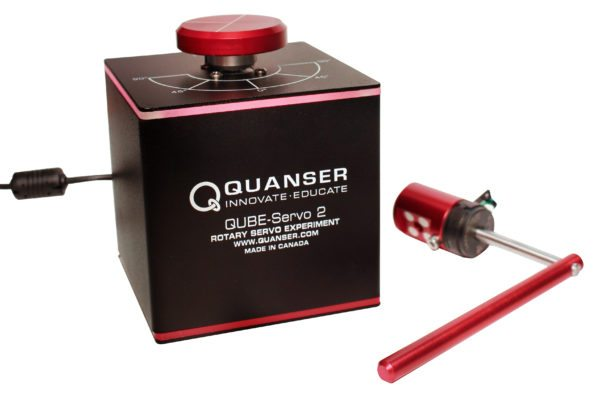
\includegraphics[scale=0.5]{QUBE-Servo_2.jpg}
%     \caption{Disque simple}
%     \label{fig:disque_simple}
%     \end{figure}


% \subsection{Vérification des paramètres du moteur}

% \subsection{Affinage des paramètres du modèle}

% \section{Pendule inverse}

% \subsection{Opencv node algorithm}

% \subsection{Obstacles node algorithm}

% \subsection{Major differences between simulation and real robot}

% \section{Conclusion and perspectives}


\end{document}
